\documentclass{article}
\usepackage[T1]{fontenc}
\usepackage{lmodern}
\usepackage{graphicx}
\usepackage{amsmath,amssymb}
\usepackage[a4paper,margin=2cm]{geometry}
\usepackage[absolute,overlay]{textpos}
\setlength{\TPHorizModule}{1mm}
\setlength{\TPVertModule}{1mm}
\usepackage[indonesian]{babel}
\usepackage{hyperref}
\setlength{\emergencystretch}{2em}
% unit: Halaman 49

\begin{document}

% === Halaman 49 (llm) ===

\vspace{118.80mm}

\begin{itemize}
    \item Berikutnya, dekripsi $C$ dengan semua semua kemungkinan nilai $K2$ (yaitu sebanyak $2^{56}$ kemungkinan kunci).
    \item Bandingkan semua hasil dekripsi ini dengan elemen di dalam tabel tadi. Jika ada yang sama, maka dua buah kunci, $K1$ dan $K2$, telah ditemukan.
    \item Tes kedua kunci ini dengan pasangan plainteks-cipherteks lain yang diketahui. Jika kedua kunci tersebut menghasilkan cipherteks atau plainteks yang benar, maka $K1$ dan $K2$ tersebut merupakan kunci yang benar
\end{itemize}

% deskripsi: Tabel perbandingan hasil enkripsi dan dekripsi untuk menemukan kunci K1 dan K2, menampilkan kolom K1, X, K2, dan X dengan beberapa nilai biner yang ditandai warna merah untuk menunjukkan kecocokan.
% bbox normalisasi: [0.5900, 0.4000, 0.9600, 0.8000]
\begin{textblock*}{77.70mm}(123.90mm,118.80mm)
\noindent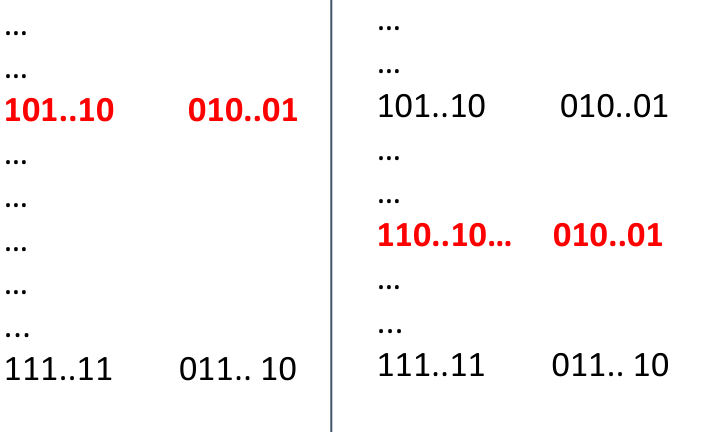
\includegraphics[width=77.70mm,height=118.80mm]{../../images/llm/page_049_img_01.png}%
\end{textblock*}

\end{document}
